% !TEX root =../thesis-letomes.tex

\chapter{Software Engineering}

The project has been defined by a relatively wide scope of disciplines that we have worked on. Mathematic derivations, astrophysics intuition, machine learning, high-performance computing, and software engineering. The last of those particularly because of the simultaneous need for rapid prototyping and strong performance characteristics. Essentially, we needed to be able to test a plethora of different ideas to answer all our questions, but since the computations are so relatively expensive, we wanted to build a few solid modules that could be treated as black boxes for our overarching purposes. Essentially, we rewrote the simulator from the precursor project from the ground up, with a focus on modularity and extensibility. This was done on basis of the model inherent in the original, to give us a consistent  with which to compare our new simulator.




\section{Software Architecture Overview}
Our system is organized as two modules with an interface between them. The top-level module is the ES algorithm and its various auxiliary functions, and the bottom level module is the orbsim module, which takes care of the astrophysics aspect; turning launch parameters into trajectories. Between them is an interface that turns machine learning parameters into astrophysic parameters, and the reverse. Visualized in \cref{fig:software_architecture}, this architecture lets us keep variable names consistent with the literature for both domains. The multidisciplinary nature of this project and its authors made this a boon.

\begin{figure}
    \centering
    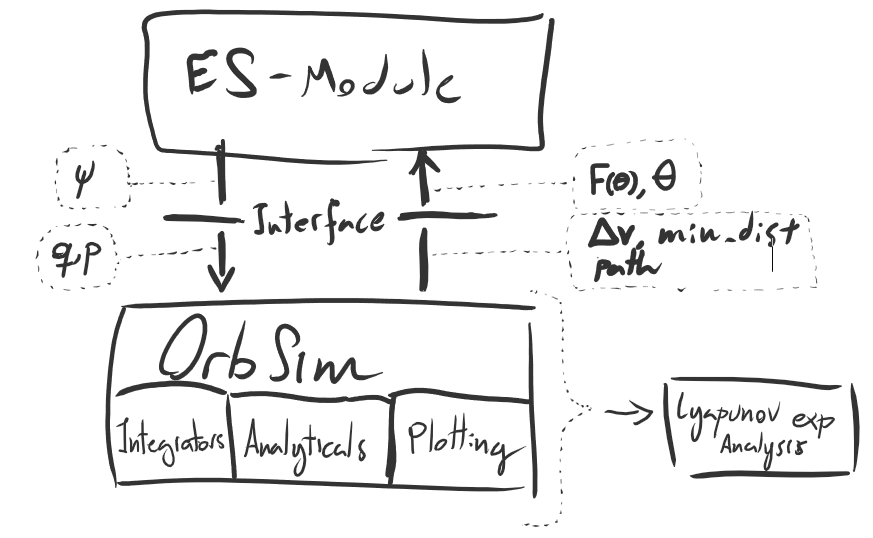
\includegraphics[width=0.76\linewidth]{fig/software_architecture}
    \caption{The architecture of the project, ES module inputs parameters to orbital simulator, which returns scores and trajectories}
    \label{fig:software_architecture}
\end{figure}

\section{Legacy Software from BSc Project}
\section{Unit Testing}
ensuring correctness of complex system with many edits taking place.
\section{Software Architecture}
\subsection{Orbsim Module}
We have arranged our code into a python module that offers us some nice modularity and extensibility, at least as far as our relatively specific problem is concerned. What follows is an explanation of the architecture of this module.

We packaged the new simulator into its own python module, installable with pip, to ensure proper reproducibility across machines and different python configurations. We then implemented the simulator into our ES framework, which we had previously developed using mock data, and tuned its hyperparameters to let it function as a decent search strategy for the lunar case. As we pursued this goal, performance became a severe issue. The ES algorithm wants to compute trajectories thousands or millions of times, and that was not feasible with each trajectory taking \SIrange{60}{300}{\second} to compute, so we delved into the simulator again in order to optimize it with regards to runtime.

\subsubsection{Abstractions}

The simulator is a numerical solver for an analytical problem, implementing algorithms that have been defined through that analysis. Thus, we have taken care to keep nomenclature consistent between the simulator and its analytical foundations. Between code and paper, if you will. This is complicated somewhat by the fact that we are applying Evolution Strategies as our search strategy, which carries with it its own set of nomenclature from the machine learning world. We have kept the two things largely separate, with the ES module interacting with the simulator through a relatively simple interface. This works fine, since ES is a black-box optimizer anyway.

\subsubsection{Simulator module}

Here, we have the interface between ES portion and simulator.

\noindent The function \texttt{launch\_sim} takes hyperparameters that the ES algorithm uses for its optimization (in the form of a decision vector \(\psi\)), reformulates them, and starts a simulation based on them. It then returns a delta-v for that single run, along with the associated saved path. That delta-v is, as mentioned before, our fitness function, so based on that result, ES can continue to do its job.

\subsubsection{Integrators module}

This contains the main loop of our simulator algorithm, along with subfunctions for the individual steps.

\subsubsection{Analyticals module}

This module contains a ton of different convenience functions that compute some intermediate equation for use in the main algorithm. They are hidden away here to reduce clutter in \texttt{Integrators.py}.

\subsubsection{Planets module}

Here, we define a planet class, which we use to store the various constants associated with a given planet. Note that we also consider the moon a planet for this purpose. We keep information such as mass and safe orbital radius here, again to simplify and improve the readability of the main algorithm. The full list of planetary constants can be seen in \todoref{Planetary constants}

\subsection{The ES module}
\begin{enumerate}
    \item hyperparameters
    \item trial and error (finding a model that worked)
\end{enumerate}

\todo{Do hyperparameters, trial and error}


The ES module conducts black-box optimization on a decision vector that describes the initial parameters for a launch. Every time the algorithm wants to find the fitness of a given point in our parameter space, it calls the orbsim module with those parameters, using the returned value as the function to minimize. The algorithm is parallelized through the use of PaGMO, which runs the ES algorithm on multiple cores independently, with many separate starting conditions.

The module defines a PyGMO \emph{problem} class, which gives the bounds and fitness function for our optimization space. The fitness function takes the decision vector \(\psi\) as argument, calls on orbsim to run a simulation with the contained parameters, and returns the result of that simulation: The \(\Delta v\) value, or if the rocket did not hit the target, how close it came at the minimum, \(d_{min}\). The fitness is a single scalar, so the fact that that scalar can mean two different things (a change in velocity or a distance) gives some problems for estimating gradients in our space. We mitigate this by penalizing an unsuccessful mission heavily, by adding an upward bias and weight, as well as squaring the result, to amplify the effect of small differences in \(d_{min}\).

We then define the ES algorithm with an \texttt{evolve} function, which executes a single run of the algorithm. This function takes a population \(\psi\): A collection of decision vectors. For each vector at step t \((\psi_{i,t})\), \texttt{evolve} creates several jittered copies \(\epsilon\) of those vectors, akin to creating a gaussian point cloud in the 3-dimensional problem space that the vectors span. Each of the points in \(\epsilon\) is then run through the fitness function, and the weighted average over \(\epsilon\) -- according to fitness score -- is deemed as the direction for the next point \(\psi_{i,t+1}\). We then take a step in that direction, modified by our learning rate \(\alpha\). This process repeats, until the algorithm has converged upon a local minimum, or until some maximum number of steps have been taken.

For the points in \(\epsilon\), we took an adaptive approach, in the interest of performance. \(\epsilon_i\) should contain enough points to get a decent estimation of the gradient around \(\psi_i\). That number is of the order \num{1e3}. This implies a large number of fitness evaluations, and with our relatively expensive fitness function, we needed to compromise a bit. We let the fitness function accept a custom limit on its runtime, and let evaluations \(F(\theta_\epsilon)\) terminate after a number of steps that was two orders of magnitude lower than that for \(F(\theta_\psi)\). For such evaluations, we also increased the error tolerance commensurately, since it would otherwise mean that those paths would be only one a fraction of  the length, which would have been completely useless.

This adaptive precision approach was a reasonable compromise, we found, since the specific error of the \(\theta_\epsilon\) paths is relatively unimportant. After all, they are only there to give an estimate of which direction improves the score. When we make a move, we select new values for \(\psi\), and conduct a full-precision fitness evaluation for it. The only worry was, that in a sufficiently chaotic system, the increased error could cause the ES algorithm to move in the wrong direction, but we estimated that to be an edge-case, solved by annealing.

This function is run in parallel on many cores, each with a different set of starting conditions \(\psi\). When all threads have finished, the best results are extracted and plotted, giving their \(\Delta v\).

Originally, we took care of parallelization with PyGMO's method of creating an archipelago, i.e a collection of islands. Each island would then run the algorithm on their own separate populations. Each island is assigned its own thread of execution. This convenient metaphor and easy implementation was the main draw of PyGMO for us, but we found that it introduced a significant performance overhead, and furthermore did not allow customization to the degree that we required. We therefore reimplemented the parallelization with less abstraction towards the end of the project.



\section{High Performance Computing}
ES uses an approach that requires a very large number of evaluations of its fitness function. 
as it relates to ES with an expensive objective function.

\todo{making the case for parallelism, given that trajectories are independent}


\subsection{Numba}

Python is a notoriously slow language, due to its paradigm of not compiling code, but simply running on the script itself; with Numba however, we can mitigate this problem, without sacrificing too much of the very high productivity that Python offers. We attempted to have Numba optimize our code for us, but found that our "proper software engineering" philosophy was preventing this from working to any meaningful effect. Numba is only able to give significant performance increases if working with basic types: Integers, Floats, Strings, and lists of those, more or less. As soon as complicated data structures are introduced into the mix, Numba drops to `object mode', where it attempts to find subsections of the function that are purely defined with basic types. This mode was useless for us simply making the code run slower due to the overhead of the compilation.

In order to get the performance increases that the problem required, we had to make some sacrifices in our idealized architecture, ditching any complicated return types, any use of exceptions and the \texttt{Planet} class that we were using to contain our data. This was a painful sacrifice, since it enabled us to simply call the algorithm with a named celestial body, and instantly have all the relevant parameters in place for computing a trajectory. Instead, we have been forced to split it into several functions with duplicated code, and a significant increase in visual and lexicographical complexity; a large reason for the redesign happening in the first place. Regrettable, but a valuable learning experience.

All this heart-wrenching work was not for nothing however, since with the pre-compilation of the symplectic Störmer-Verlet algorithm in place, we were seeing speedups of a factor 2-300. 

Once we had this architecture in place, and giving the same results as the original simulator, we built extensions to it to cover the martian travel case unique to this project.\todo{More about software architecture / numba optimization when mars is working}

\subsection{CUDA}

We attempted to gain additional performance from our simulator, we tried to run it on GPUs. Given that the fitness evaluations are completely independent in ES, it is a great candidate for massive parallelization. This is also doable with Numba, but requires an even more granular refactoring of the simulator code, and conscious management of data transfer between CPU and GPU, since the communication overhead associated with GPU work can very easily eclipse the performance gained by the massive parallelization. We attempted to make the necessary changes, but in the end we could not get it to work, and decided that the medium level of parallelization that we could achieve easily would have to be enough. The HPC CPU clusters have two \SI{2.8}{\GHz} 10-core Intel Xeon processors, so they are nothing to scoff at by themselves. Still, performance has been a limiting factor for the types and number of experiments we could do on the ML front, so in the future, we would like to pursue the GPU angle further.



\section{GPU programming with CUDA}
massive parallelism vs. data transfer overhead.
